\documentclass[10pt,conference,a4paper]{IEEEtran}
\usepackage{amsmath}
\usepackage[utf8]{inputenc}
\usepackage{tikz}
\usepackage{xcolor}
\usetikzlibrary{arrows.meta, decorations.pathreplacing, fit, positioning}

\begin{document}

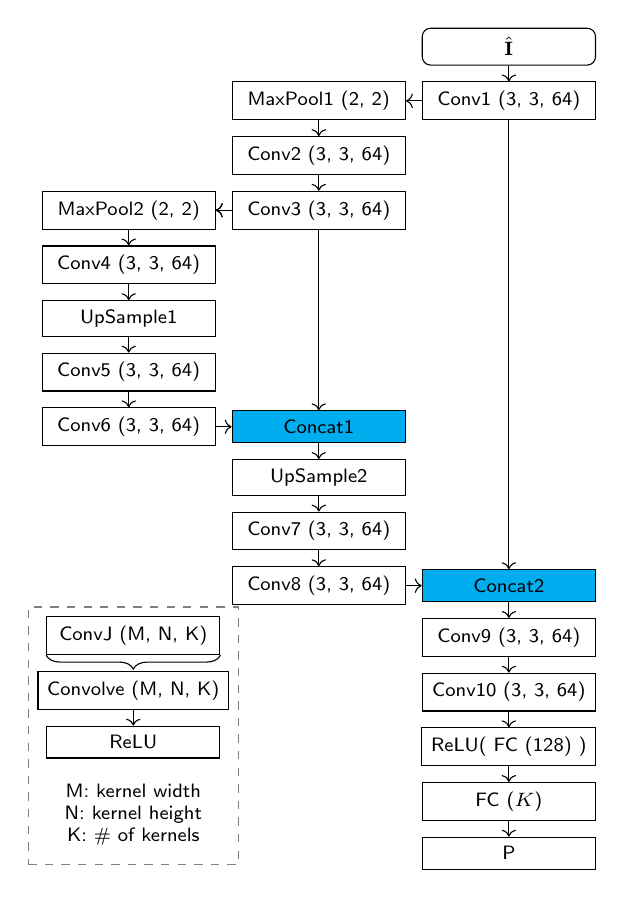
\begin{tikzpicture}[node distance=.2cm, align=center, base/.style = {rectangle, draw=black, minimum width=2.2cm, minimum height=.15cm, text centered, font=\sffamily\scriptsize},
  inout/.style = {base, rounded corners=3pt},
  layer/.style = {base}]
    \node (img) [inout]{\(\hat{\mathbf{I}}\)};
    \node (conv1) [layer, below=of img] {Conv1 (3, 3, 64)};
    \node (pool1) [layer, left=of conv1] {MaxPool1 (2, 2)};
    \node (conv2) [layer, below=of pool1] {Conv2 (3, 3, 64)};
    \node (conv3) [layer, below=of conv2] {Conv3 (3, 3, 64)};
    \node (pool2) [layer, left= of conv3] {MaxPool2 (2, 2)};
    \node (conv4) [layer, below=of pool2] {Conv4 (3, 3, 64)};
    \node (up1) [layer, below=of conv4] {UpSample1};
    \node (conv5) [layer, below=of up1] {Conv5 (3, 3, 64)};
    \node (conv6) [layer, below=of conv5] {Conv6 (3, 3, 64)};
    \node (concat1) [layer, right=of conv6, fill=cyan] {Concat1};
    \node (up2) [layer, below=of concat1] {UpSample2};
    \node (conv7) [layer, below=of up2] {Conv7 (3, 3, 64)};
    \node (conv8) [layer, below=of conv7] {Conv8 (3, 3, 64)};
    \node (concat2) [layer, right=of conv8, fill=cyan] {Concat2};
    \node (conv9) [layer, below=of concat2] {Conv9 (3, 3, 64)};
    \node (conv10) [layer, below=of conv9] {Conv10 (3, 3, 64)};
    \node (fc1) [layer, below=of conv10] {ReLU( FC (128) )};
    \node (fc2) [layer, below=of fc1] {FC (\(K\))};
    \node (output) [layer, below=of fc2] {P};
    \node (convLayer) [layer, below left=of conv8] {ConvJ (M, N, K)};
    \node (convolution) [layer, below=of convLayer] {Convolve (M, N, K)};
    \node (relu) [layer, below=of convolution] {ReLU};
    \node (descr) [font=\sffamily\scriptsize, below=of relu] {M: kernel width\\N: kernel height\\K: \# of kernels};
    \node [fit=(convLayer)(convolution)(relu)(descr), draw, gray, dashed]{};
    \begin{scope}[all/.style={width=2mm, length=2mm}]
      \draw[->] (img) -- (conv1);
      \draw[->] (conv1) -- (pool1);
      \draw[->] (conv1) -- (concat2);
      \draw[->] (pool1) -- (conv2);
      \draw[->] (conv2) -- (conv3);
      \draw[->] (conv3) -- (pool2);
      \draw[->] (conv3) -- (pool2);
      \draw[->] (conv3) -- (concat1);
      \draw[->] (pool2) -- (conv4);
      \draw[->] (conv4) -- (up1);
      \draw[->] (up1) -- (conv5);
      \draw[->] (conv5) -- (conv6);
      \draw[->] (conv6) -- (concat1);
      \draw[->] (concat1) -- (up2);
      \draw[->] (up2) -- (conv7);
      \draw[->] (conv7) -- (conv8);
      \draw[->] (conv8) -- (concat2);
      \draw[->] (concat2) -- (conv9);
      \draw[->] (conv9) -- (conv10);
      \draw[->] (conv10) -- (fc1);
      \draw[->] (fc1) -- (fc2);
      \draw[->] (fc2) -- (output);
      \draw[->] (convolution) -- (relu);
      \draw[decorate, decoration={brace, mirror, amplitude=5pt}] (convLayer.south west) -- (convLayer.south east);
    \end{scope}
  \end{tikzpicture}

\end{document}